\documentclass{../industrial-development}
\graphicspath{{10-quality-assurance/}}

\title{Обеспечение качества ПО}
\author{Глазовский Александр, Совин Алексей}
\date{}

\begin{document}
	
	\begin{frame}
		\titlepage
	\end{frame}
	
	
	
	\section{Понятие качества ПО}
	\begin{frame} \frametitle{Понятие качества ПО}
		\begin{block}{}
			\alert{Качество программного обеспечения} --- это совокупность характеристик ПО, относящихся к его способности удовлетворять установленные и предполагаемые потребности пользователя
		\end{block}
		\begin{itemize}
			\item Функциональность (Functionality)
			\item Надежность (Reliability)
			\item Удобство использования (Usability)
			\item Эффективность (Efficiency)
			\item Удобство сопровождения (Maintainability)
			\item Портативность (Portability)
		\end{itemize}
	\end{frame}
	
	\begin{frame} \frametitle {Функциональность}
		\begin{block}{}
			\alert{Функциональность} --- способность ПО в определенных условиях решать задачи, нужные пользователям
		\end{block}
		\begin{itemize}
			\item Функциональная пригодность (suitability) --- способность решать нужный набор задач
			\item Точность (accuracy) --- способность выдавать нужные результаты
			\item Способность к взаимодействию (interoperability) --- способность взаимодействовать с набором других систем
			\item Соответствие стандартам и правилам (compliance)
			\item Защищенность (security) --- способность предотвращать неавторизированный доступ к данным и программам
		\end{itemize}
	\end{frame}
	
	\begin{frame} \frametitle {Надежность}
		\begin{block}{}
			\alert{Надежность} ---  способность  ПО  поддерживать  определенную  работоспособность в заданных условиях 
		\end{block}
		\begin{itemize}
			\item Зрелость, завершенность (maturity) --- величина, обратная частоте отказов ПО
			\item Устойчивость к отказам (fault tolerance) --- способность поддерживать заданный уровень работоспособности при отказах и нарушениях правил взаимодействия с окружением
			\item Способность к восстановлению (recoverability) --- способность восстанавливать определенный уровень работоспособности и целостность данных после отказа
			\item Соответствие стандартам надежности (reliability compliance)
		\end{itemize}
	\end{frame}
	
	\begin{frame} \frametitle {Удобство использования}
		\begin{block}{}
			\alert{Удобство использования} --- способность ПО быть удобным в обучении и использовании, а также привлекательным для пользователей 
		\end{block}
		\begin{itemize}
			\item Понятность (understandability) --- показатель, обратный к усилиям, затрачиваемым пользователями на восприятие основных понятий ПО
			\item Удобство обучения (learnability) --- показатель, обратный усилиям, затрачиваемым пользователями на обучение работе
			\item Удобство работы (operability) --- показатель, обратный усилиям, предпринимаемым пользователями для решения своих задач с помощью ПО
			\item Привлекательность (attractiveness) --- способность ПО быть привлекательным для пользователей
		\end{itemize}
	\end{frame}
	
	\begin{frame} \frametitle {Эффективность}
		\begin{block}{}
			\alert{Эффективность} --- способность ПО при заданных условиях обеспечивать необходимую работоспособность по отношению к выделяемым для этого ресурсам
		\end{block}
		\begin{itemize}
			\item Временная эффективность (time behaviour) --- способность ПО выдавать ожидаемые результаты и обеспечивать передачу необходимого объема данных за отведенное время
			\item Эффективность использования ресурсов (resource utilisation) --- способность решать нужные задачи с использованием определенных объемов ресурсов
		\end{itemize}
	\end{frame}
	
	\begin{frame} \frametitle {Удобство сопровождения}
		\begin{block}{}
			\alert{Удобство сопровождения} --- удобство проведения всех видов деятельности, связанных с сопровождение программ
		\end{block}
		\begin{itemize}
			\item Анализируемость (analyzability) --- удобство проведения анализа ошибок, а также удобство анализа необходимости изменений и их возможных последствий
			\item Удобство внесения изменений (changeability) --- показатель, обратный трудозатратам на выполнение необходимых изменений
			\item Стабильность (stability) --- показатель, обратный риску возникновения неожиданных эффектов при внесении необходимых изменений
		\end{itemize}
	\end{frame}	
	
	\begin{frame} \frametitle {Переносимость}
		\begin{block}{}
			\alert{Переносимость} --- способность ПО сохранять работоспособность при переносе из одного окружения в другое
		\end{block}
		\begin{itemize}
			\item Адаптируемость (adaptability) --- способность ПО приспосабливаться к различным окружениям без проведения для этого специальных действий
			\item Удобство установки (installability) --- способность ПО быть установленным в определенном окружении
			\item Способность к сосуществованию (coexistence) --- способность ПО сосуществовать с другими программами, деля с ними ресурсы
		\end{itemize}
	\end{frame}	
	
	\section{Понятие обеспечения качеством}
	\begin{frame} \frametitle {Обеспечение качества}
		\begin{block}{}
			\alert{Обеспечение качества} --- это совокупность мероприятий, охватывающих все технологические этапы разработки, выпуска и эксплуатации ПО, предпринимаемых на разных стадиях жизненного цикла, для обеспечения требуемого уровня качества выпускаемого продукта	
		\end{block}
		\begin{itemize}
			\item Верификация --- процесс оценки системы или её компонентов с целью определения, удовлетворяют ли результаты текущего этапа разработки условиям, сформированным в начале этого этапа
			\item Валидация --- это определение соответствия разрабатываемого ПО ожиданиям и потребностям пользователя, требованиям к системе
		\end{itemize}
	\end{frame}
	\begin{frame} \frametitle {Роль QA}
	\begin{itemize}
		\item Выявляние слабых мест и несоответствий в продукте на всех этапах разработки
		\item Помощь в определение требований к проекту
		\item Предоставление информации о качестве продукта
		\item Тестирование продукта на протяжении всех фаз жизненного цикла разработки системы 
	\end{itemize}
\end{frame}	
	
	\begin{frame} \frametitle{Иерархия процессов QA}
		\centerline{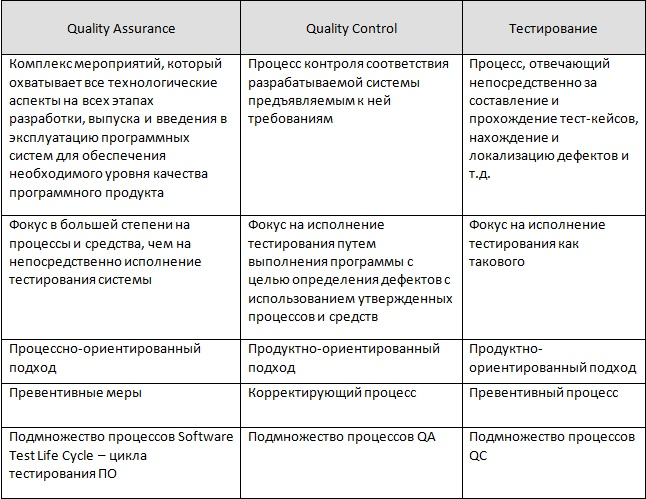
\includegraphics[height=0.7\textheight]{QA_QC.png}}
	\end{frame}
	
	\begin{frame} \frametitle{Иерархия процессов QA}
		\begin{itemize}
			\item Quality Assurance обеспечивает правильность и предсказуемость процесса 
			
			\item Quality Control --- гарантирует соответствие требованиям (поиск ошибок и их устранение).
			
			\item Тестирование --- это сбор статистических данных и внесение их в документы, созданные в рамках QC-процесса.
		\end{itemize}
	\end{frame}
	
		
\section{QA в жизненном цикле продукта}
	\begin{frame} \frametitle{Сбор требований}
		\begin{itemize}
			\item Анализ и принятие решения о том, совместимы ли между собой требования, и могут ли они быть реализованы в рамках одной системы
			\item Оценка того, какие решения будут работать, а какие --- нет
			\item Планирование необходимых методов тестирования
			\item Обзор требований рынка и пользователей
		\end{itemize}
	\end{frame}
\lecturenotes
В течение этого этапа QA работают вместе с бизнес-аналитиками с целью выяснить, какой программный продукт может удовлетворить потребности пользователя. По сути, они проверяют, нужен ли продукт пользователям и рынку. Очень важно собрать отзывы пользователей, чтобы узнать, чего не хватает или что может быть улучшено для обеспечения лучшего пользовательского опыта
	
	\begin{frame} \frametitle{Планирование тестирования}
			На этом этапе QA определяют стратегию тестирования. Под определением стратегии имеется в виду оценка времени и усилий для всего проекта. После анализа требований QA создают документ, известный как тест-план. Он включает в себя ожидаемые результаты проекта, его масштаб и цель, а также определяет среду тестирования.
			Без этого этапа процесс тестирования был бы полон неожиданных препятствий и непредвиденных обстоятельств. Чтобы дальнейшие этапы следовали строгой последовательности действий, QA должен составить и задокументировать план действий. В противном случае процесс может получиться неуклюжим
	\end{frame}
	
	\begin{frame} \frametitle{Разработка тестов}
		\begin{itemize}
			\item Создание тест-кейсов
			\item Создание плана проведения тестирования
			\item Определение критериев приемлимости тестирования
		\end{itemize}
	Когда у нас есть тест-план, мы можем приступить к настройке среды тестирования и созданию тест-кейсов. Тест-кейс --- это набор шагов, которые нужно выполнить, чтобы удостовериться, что в продукте нет ошибок и он работает согласно требованиям. После этого можно думать о критерии приемлемости — техническом стандарте, которому должен соответствовать программный продукт, чтобы считаться успешным.
	\end{frame}
	
	\begin{frame} \frametitle{Выполнение тестов}
	Этот этап многие считают единственной задачей QA --- выполнение всех тест-кейсов по плану. Если какая-то часть системы работает хорошо, мы отмечаем её как прошедшую тестирование. Таким образом мы можем удостовериться, что ничего не пропустим и на выходе получим качественный продукт.
	
	Если тест-кейс прошёл неудачно, значит в коде есть ошибка, и QA отправляют отчёт разработчикам, чтобы они проверили, что не так
	\end{frame}
	
	\begin{frame} \frametitle{Отчёт о результатах}
	После тестирования продукта наступает время обсуждения, что было хорошо, а что не очень, для улучшения дальнейших циклов тестирования. Чтобы обеспечить быстрое исправление ошибок без каких-либо недопониманий со стороны разработчиков, каждая обнаруженная проблема должна быть хорошо задокументирована. Позже мы посмотрим на наиболее распространённые методы, которые используют QA для тестирования продукта с разных точек зрения.
	
	Цикл тестирования --- это частота, с которой мы проводим эти пять этапов тестирования
	\end{frame}
\section{Роли в QA}
	\begin{frame} \frametitle{Руководитель QA}
		\begin{itemize}
			\item Действует как точка контакта для межведомственного и внутриведомственного взаимодействия
			\item Представляет команду тестирования программного обеспечения, а также обеспечивает отношения с клиентами
			\item Определяет бюджет тестирования и его график
			\item Определяет действий по тестированию для других членов команды
			\item Планирует весь процесс тестирования
			\item Определяет действий по тестированию для других членов команды
		\end{itemize}
	\end{frame}
	\begin{frame} \frametitle{Руководитель QA}
		\begin{itemize}
			\item Проверяет доступность ресурсов для выполнения действий по тестированию
			\item Обеспечивает синхронизацию процесса тестирования с разработкой программного обеспечения
			\item Подготавливает отчет о состоянии тестирования
			\item Планирует тестирование до и после встреч по тестированию
		\end{itemize}
	\end{frame}
	\begin{frame} \frametitle{Руководитель тестирования}
		\begin{itemize}
			\item Техническая экспертиза, связанная с программой и подходом к тестированию
			\item Подготовка отчетов текущего состояния
			\item Проверка качества требований тестирования
			\item Помощь команде тестирования программного обеспечения
			\item Реализация процесса тестирования
		\end{itemize}
	\end{frame}
	\begin{frame} \frametitle{Тестирование пользовательского интерфейса}
		\begin{itemize}
			\item Разработка сценариев тестирования пользовательского интерфейса
			\item Администрирование процесса пользовательского интерфейса
			\item Разработка документации тестового продукта
			\item Участие в прохождении тестовой процедуры
		\end{itemize}
	\end{frame}
	\begin{frame} \frametitle{Ручное тестирование}
		\begin{itemize}
			\item Использование связанных данных тестирования для проектирования и разработки процедур и контрольных примеров
			\item Выполнение тестовых процедур вручную
			\item Контроль над прохождением тестовой процедуры
			\item Соответствие установленным стандартам тестирования
		\end{itemize}
	\end{frame}
	\begin{frame} \frametitle{Автоматизированное тестирование}
		\begin{itemize}
			\item Проектирование и разработка процедур тестирования на основе требований
			\item Контроль над прохождением тестовой процедуры
			\item Выполнение тестов
			\item Подготовка отчетов
		\end{itemize}
	\end{frame}
	\begin{frame} \frametitle{Тестирование сети}
		\begin{itemize}
			\item Выполнение тестирования сети, базы данных и промежуточного программного обеспечения
			\item Разработка нагрузочных и стресс-тестовых конструкций, кейсов и процедур
			\item Внедрение инструментов мониторинга производительности на постоянной основе
			\item Проведение нагрузочных и стресс-тестовых процедур
		\end{itemize}
	\end{frame}
	\begin{frame} \frametitle{Тестирование библиотек и конфигурации}
		\begin{itemize}
			\item Управление изменениями тестовых скриптов
			\item Ведение контроля версий тестовых скриптов
			\item Поддержка библиотеки повторного использования тестовых скриптов
			\item Создание тестовых сборок
		\end{itemize}
	\end{frame}
	\section{Основные показатели процесса QA}
	\begin{frame} \frametitle{Какими должны быть метрики?}
		\begin{itemize}
			\item Основная цель любой метрики --- это улучшение процесса разработки и самого программного продукта. Метрика позволяет увидеть, в какой точке на пути к целям мы находимся в данный момент, приближаемся к ним или удаляемся, достигаются ли критерии успешности.
			\item Метрики не должны существовать ради самого процесса измерения. Необходимо использовать только те метрики, которые действительно имеют практическое значение и будут влиять на дальнейшее развитие продукта или оптимизацию процесса. Отсюда следует простое правило --- сначала нужно определить зоны для изменения(улучшения), а потом решать, как их оценивать.
		\end{itemize}
	\end{frame}

	\begin{frame} \frametitle{Основные группы метрик для QA}
		\begin{itemize}
			\item Требования к разрабатываемому ПО.
			\item Качество разрабатываемого продукта.
			\item Возможности команды QA.
			\item Качество работы команды тестирования.
			\item Обратная связь и удовлетворенность продуктом.
		\end{itemize}
	\end{frame}
	\begin{frame} \frametitle{Требования к разрабатываемому ПО}
		\begin{itemize}
			\item Тестовое покрытие требования 
			\item Степень взаимосвязанности требований
			\item Коэффициент стабильности требований
		\end{itemize}
	\end{frame}

	\begin{frame} \frametitle{Качество разрабатываемого продукта}
		\begin{itemize}
			\item Плотность дефектов
			\item Коэффициент регрессии
			\item Коэффициент повторно открытых дефектов
		\end{itemize}
	\end{frame}

	\begin{frame} \frametitle{Возможности и эффективность команды QA}
		\begin{itemize}
			\item Скорость работы (velocity) команды QA
			\item Среднее время жизни дефекта
			\item Коэффициент повторно открытых дефектов
		\end{itemize}
	\end{frame}

	\begin{frame} \frametitle{Качество работы команды тестирования}
		\begin{itemize}
			\item Эффективность тестов и тестовых наборов
			\item Коэффициент ошибок, пропущенных на продуктив
			\item Реальное время работы команды QA
			\item Точность оценки времени по областям/видам/типам работ
		\end{itemize}
	\end{frame}

	\begin{frame} \frametitle{Обратная связь и удовлетворенность пользователей}
		\begin{itemize}
			\item Удовлетворенность пользователей ИТ сервисом
			\item Удовлетворенность пользователей продуктом
			\item Вовлеченность стейкхолдеров
		\end{itemize}
	\end{frame}

	\begin{thebibliography}{99}
		\bibitem{SQA-Galin} Galin, Daniel, Software quality assurance: from theory to implementation / Daniel Galin, 2004."--- 590с.: ил.
	\end{thebibliography}
	
\end{document}